\section{Physics Object Definition and Preselections}
\label{sect:objdef}
This section, describes the physics objects used in this analysis. 
\subsection{PF Jets}
\begin{itemize}
\item PF jets with $p_T>20$ GeV and $|\eta|<2.4$ are kept for the analysis.
\item Jets are required to pass loose pf-jet id cuts listed below:
\begin{itemize}
\item Number of constituents $>$ 1,
\item Neutral hadronic fraction $<$ 0.99,
\item Neutral electromagnetic fraction $<$ 0.99,
\item Charged hadronic fraction $>$ 0,
\item Charged electromagnetic fraction $<$ 0.99,
\item Charged multiplicity $>$ 0.
\end{itemize}
\end{itemize}
\subsection{PF Electrons}
\begin{itemize}
\item PF electrons with $p_T>10$ GeV and $|\eta|<2.4$ are selected with ECAL gap veto.
\item Electrons are required to pass cut-based electron id cuts corresponding to VBTF 95 working point, which is used for veto~\cite{eIDs}. These set of cuts contain the requirements on $|d0|<0.04$ cm and $|dz|<0.2$ cm, for which both of them are calculated with respect to the primary vertex. 
\item Combined relative PF isolation below 0.15.
\end{itemize}
\subsection{PF Muons}
\begin{itemize}
\item PF muons with $p_T>10$ GeV and $|\eta|<2.4$ are selected, which are asked to be global muons.
\item Normalized $\chi^2$ is required to be below 10.
\item At least one valid track hit and at lease one valid pixel hit is required.  
\item Number of chambers with matched segments is required to be greater than one and number of silicon layers should be above 5. 
\item Cuts on the $|d0|<0.2$ cm and the $|dz|<0.5$ cm, both with respect to the primary vertex, are applied.
\item Combined relative PF isolation below 0.2.
\end{itemize}
\subsection{PF Taus}
\label{sec:taus}
In this note taus always mean hadronically decaying taus, unless stated otherwise.
\begin{itemize}
\item Hadron Plus Strip (HPS) algorithm identified PF-taus
\item $p_\mathrm{T} > 20$ GeV and  $|\eta| <$ 2.3
\item A decay into one or three prongs, plus eventually a $\pi^0$, is required
\item Loose Electron Rejection: electron pion MVA discriminator $< 0.6$
\item Tight Muon Rejection: Tau Lead Track not matched to chamber hits, and no DT, CSC or RPC Hits in last 2 stations, and large enough energy deposit in ECAL + HCAL in 1 prong + 0 strip decay mode ($\sum$(ECAL+HCAL) $> 0.2 \cdot p_{\mathrm{T}}$.
\item Loose Isolation ($\Delta\beta$-corrected): $\Delta\beta$-corrected $\sum p_\mathrm{T}$ of PF charged and PF gamma isolation candidates ($p_\mathrm{T} > 0.5$ GeV) less than 2 GeV (in a cone of $\Delta R = 0.3$ around the tau axis), requiring 3 hits on tracks of charged isolation candidates.
\end{itemize}

\subsection{\texorpdfstring{PF \met}{PF MET}}
\begin{itemize}
\item Type1 corrected PF \met is used.
\end{itemize}
\subsection{Jet/MET Smearing}
\label{subsect:smearing}
Simulated events show discrepancies with data specially in $\met$ and $M_{T2}$ distributions. As shown in Figure~\ref{fig:metmtpresme}, the data over MC shows a trend rather than fluctuating differences.\\
\begin{figure}[!h]
 \begin{center}$
 \begin{array}{cc} 
	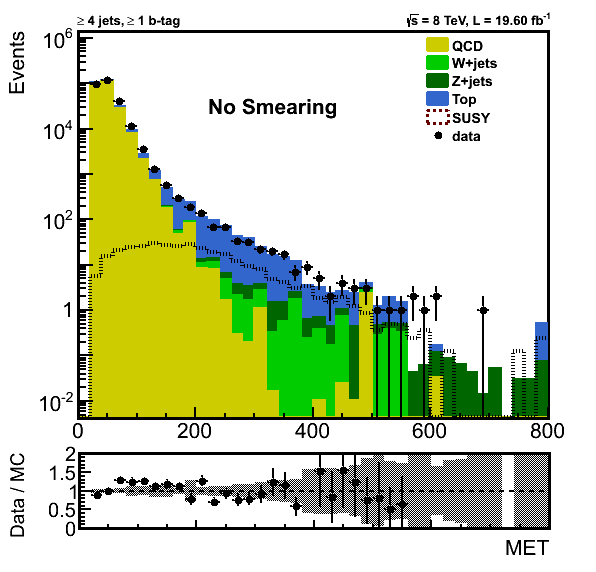
\includegraphics[angle=00,width=0.40\textwidth]{figs/METNoSmearing.png} & 
	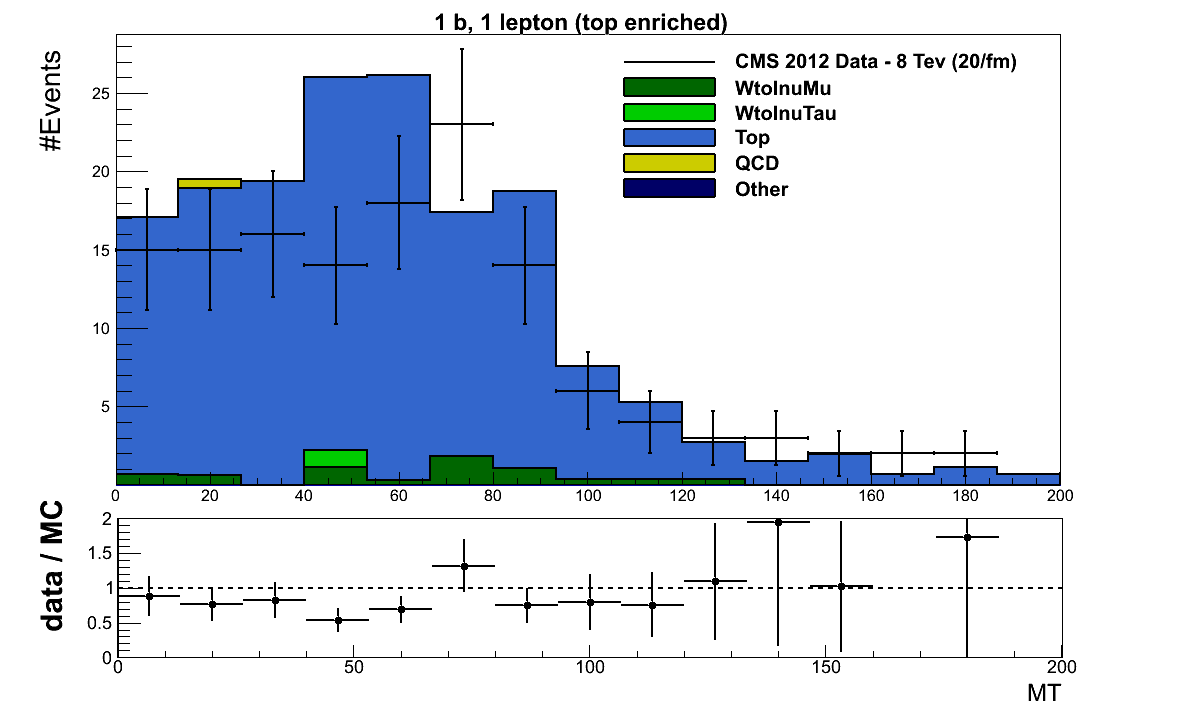
\includegraphics[angle=00,width=0.40\textwidth]{figs/MT2NoSmearing.png}\\
	\mbox{\small{a}} & \mbox{\small{b}}\\
	\end{array}$ 
  \caption{The distribution of $\met$ (a) and $M_{T2}$ (b) before smearing.}
  \label{fig:metmtpresme}
 \end{center}
\end{figure}
The energy of jets and $\met$ in simulation are calibrated based on data. There are however residual differences between data and simulation which are not covered by those corrections. Such differences could be improved by altering the jet energy resolution to match the data and correcting the $\met$ accordingly. The CMS official recipe is followed to for the jet-$\met$ smearing. Figure~\ref{fig:metmtpostsme} illustrates the improvement achieved after smearing in $\met$ and $M_{T2}$ distributions. Smeared jets and $\met$ are used in event selection and in the rest of the analysis.
\begin{figure}[!h]
 \begin{center}$
 \begin{array}{cc} 
	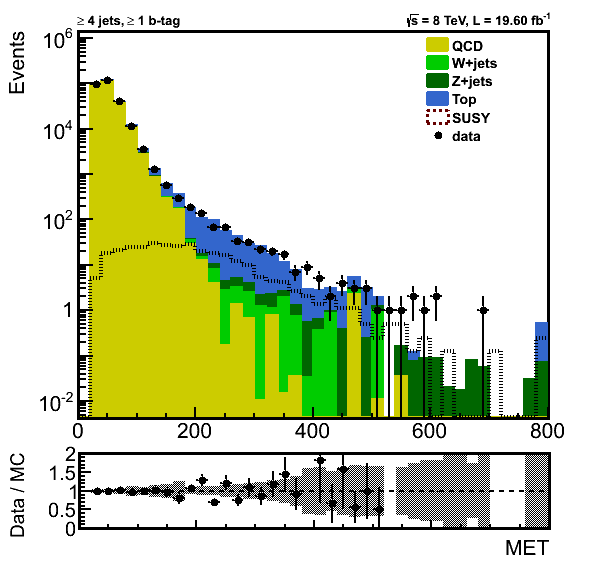
\includegraphics[angle=00,width=0.40\textwidth]{figs/METSmearedJetMET.png} & 
	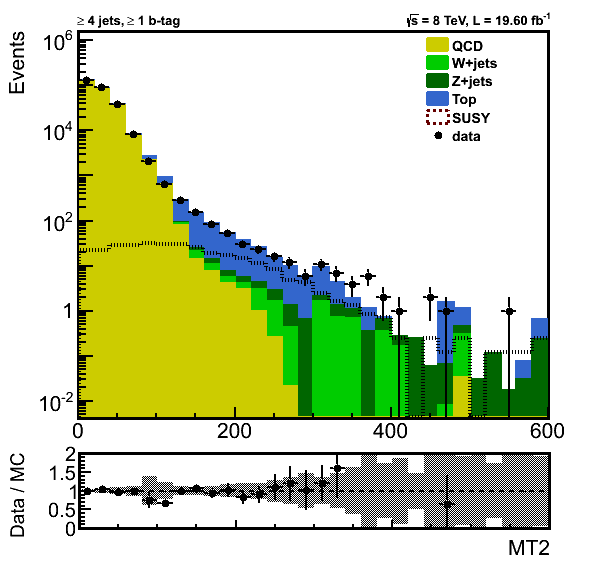
\includegraphics[angle=00,width=0.40\textwidth]{figs/MT2SmearedJetMET.png}\\
	\mbox{\small{a}} & \mbox{\small{b}}\\
	\end{array}$ 
  \caption{The distribution of $\met$ (a) and $M_{T2}$ (b) after smearing.}
  \label{fig:metmtpostsme}
 \end{center}
\end{figure}

\subsection{Preselection}
\label{subsect:presel}
\begin{itemize}
\item At least one good vertex, with $\rho<2$ cm and $\abs z<24$ cm and Ndof $>4$ is requested.
\item There are some cleaning cuts which are applied against instrumental effects, including those listed below:
\begin{itemize}
\item An isolation based HBHE noise filter is applied,
\item Events identified as beam halo are filtered.
\end{itemize}
\end{itemize}

\subsection{MT2b Cuts}
\label{subsect:mt2bcuts}
This section provides a review on the cuts which are started with to study the triggers. This set of cuts are those mainly used in the $\rm MT2b$ analysis~\cite{MT2_2011}. Once the trigger is fixed, the optimized set of selection cuts which are used in the main stream of the current analysis will be described in detail in Section~\ref{sect:cuts}.
\begin{itemize}
\item The preselection cuts which was outlined in Section~\ref{subsect:presel}.
\item At least 4 jets with $p_T>40$ GeV and $\abs\eta<2.4$ are required which are asked to pass loos pf-jet id cuts.
\item The leading jet-$p_T$ should be greater than $150$ GeV.
\item It is also required that all jets with $p_T>50$ GeV to pass loose pf-jet id cuts. Events with non-idetified high $p_T$ jets are discarded.
\item At least one b-quark jet is requested with $p_T>20$ GeV within the tracker acceptance, which is tagged by the Simple Secondary Vertex algorithm with a tight working point.
\item The difference between \met and the vectorial $p_T$ sum of the selected jets, electrons and muons, hereafter referred to as VectorSumPt, should be below $70$ GeV.
\item \met is required to be greater than $30$ GeV.
\item The minimum $\Delta\phi$ between \met and the four leading jets, hereafter referred to as \mindphifour, should be greater than $0.3$. There is no requirement on the id or $p_T$ of the jets when looking for the minimum azimuthal angle between \met and jets.
\item A cut on \mttwo $>$ 125 GeV is applied.
\item Leptons, being either electrons or muons, are vetoed.
\end{itemize}


